%clients

\subsection{Analyse}
\subsubsection{ Diagramme de cas d'utilisation "G\'{e}rer un client"}
\begin{figure}[H]
\center
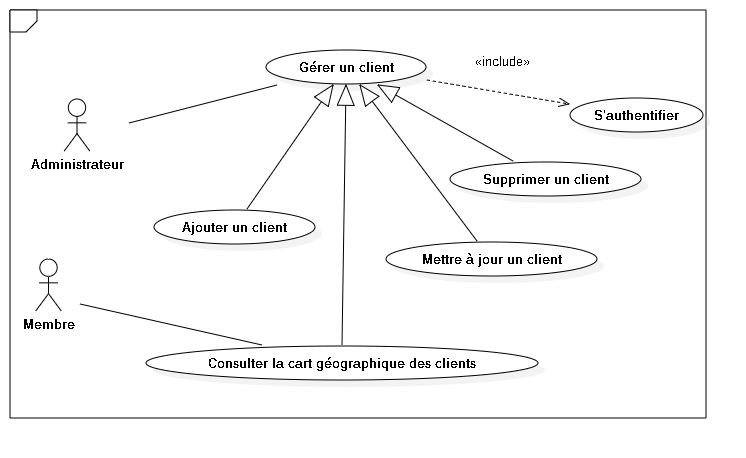
\includegraphics[width=13cm,height=8cm]{./figures/ucC.png}
\caption{G\'{e}rer un client.}
\end{figure}

\newpage
\subsection{Conception}
\subsubsection{Le sc\'{e}nario \guillemotleft{} Cr\'{e}ation d'un client\guillemotright{}}
Le diagramme de s\'{e}quence \guillemotleft{} Ajout d'une t\^{a}che \guillemotright{} pr\'{e}sente le s\'{e}quencement
des interactions entre Administrateur, Application et Base de donn\'{e}es (BD).

\begin{figure}[H]
\center
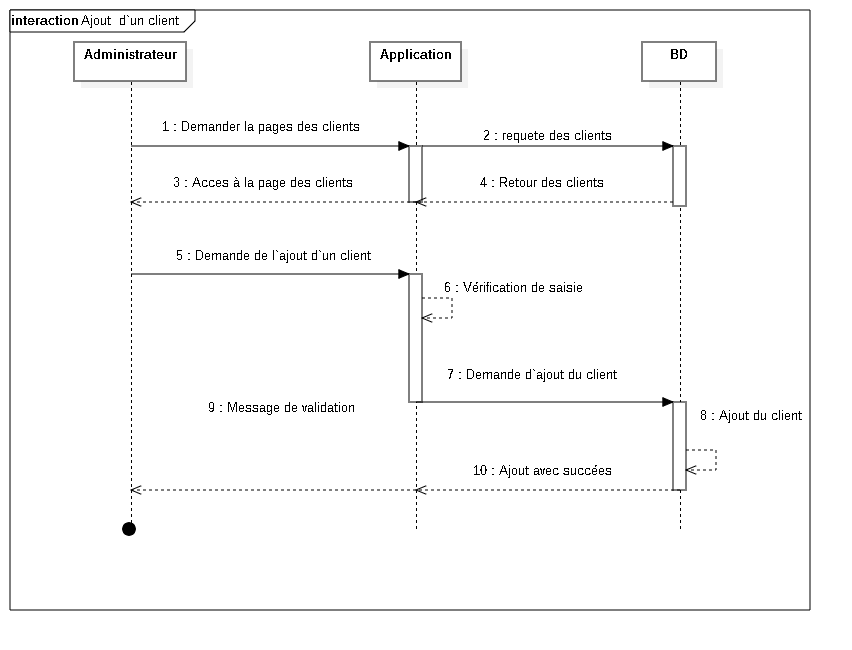
\includegraphics[width=14cm,height=9cm]{./figures/seq/F.png}
\caption{Cr\'{e}ation d'un client.}
\end{figure}



\subsubsection{Le sc\'{e}nario \guillemotleft{} Consultation de la carte g\'{e}ographique des clients\guillemotright{}}
Le diagramme de s\'{e}quence \guillemotleft{} Ajout d'une t\^{a}che \guillemotright{} pr\'{e}sente le s\'{e}quencement
des interactions entre Administrateur, Application et Base de donn\'{e}es (BD).


\newpage
\subsection{Sch\'{e}ma}
Le Schéma de la table ”customers” est présenté par la Table 3.2



\begin{table}

\begin{tabular}{|l|l|l|l|l|l|}
\hline
Field            & Type          & Null & Key & Default            & Extra            \\
\hline
id               & int(11)       & NO   & PRI & NULL               & auto\_increment  \\
\hline
name             & varchar(45)   & YES  &     & NULL               &                  \\
\hline
phone            & varchar(45)   & YES  &     & NULL               &                  \\
\hline
address          & varchar(1000) & YES  &     & NULL               &                  \\
\hline
email            & varchar(50)   & YES  &     & NULL               &                  \\
\hline
longitude        & double        & YES  &     & NULL               &                  \\
\hline
latitude         & double        & YES  &     & NULL               &                  \\
\hline
subscriptionDate & datetime      & YES  &     & CURRENT\_TIMESTAMP &                  \\
\hline
\end{tabular}
\centering
\caption{Customers}
\end{table}


\subsection{Test}


\begin{figure}[H]
\center
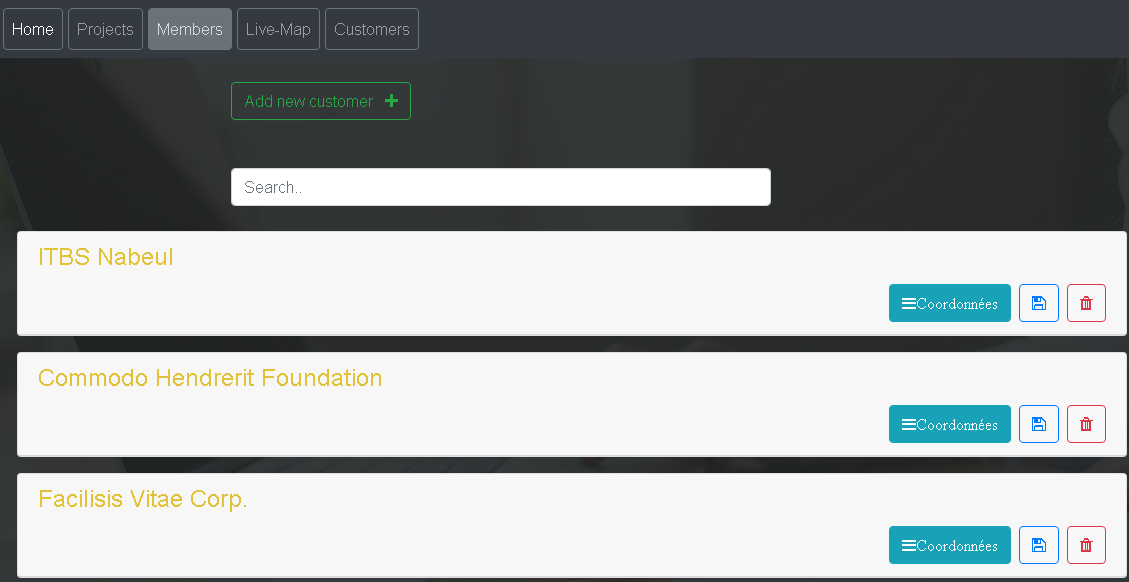
\includegraphics[width=11cm,height=7cm]{./figures/pres/cc1.png}
\caption{Gestion des clients.1.}
\end{figure}




\begin{figure}[H]
\center
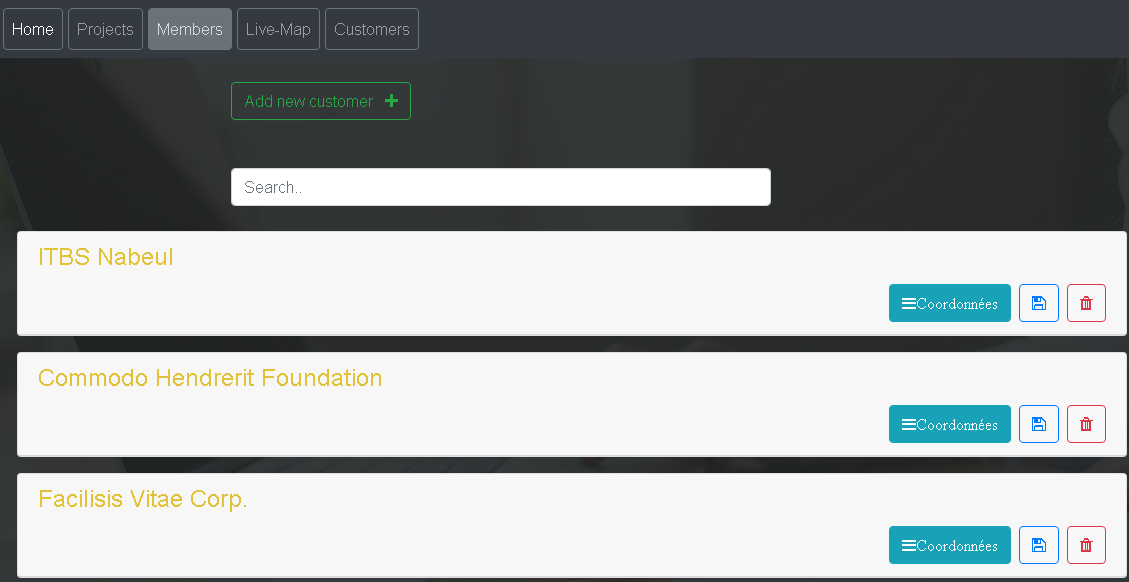
\includegraphics[width=11cm,height=7cm]{./figures/pres/cc1.png}
\caption{Gestion des clients.2.}
\end{figure}

\subsection{Consultation carte g\'{e}ographique des clients}


\begin{figure}[H]
\center
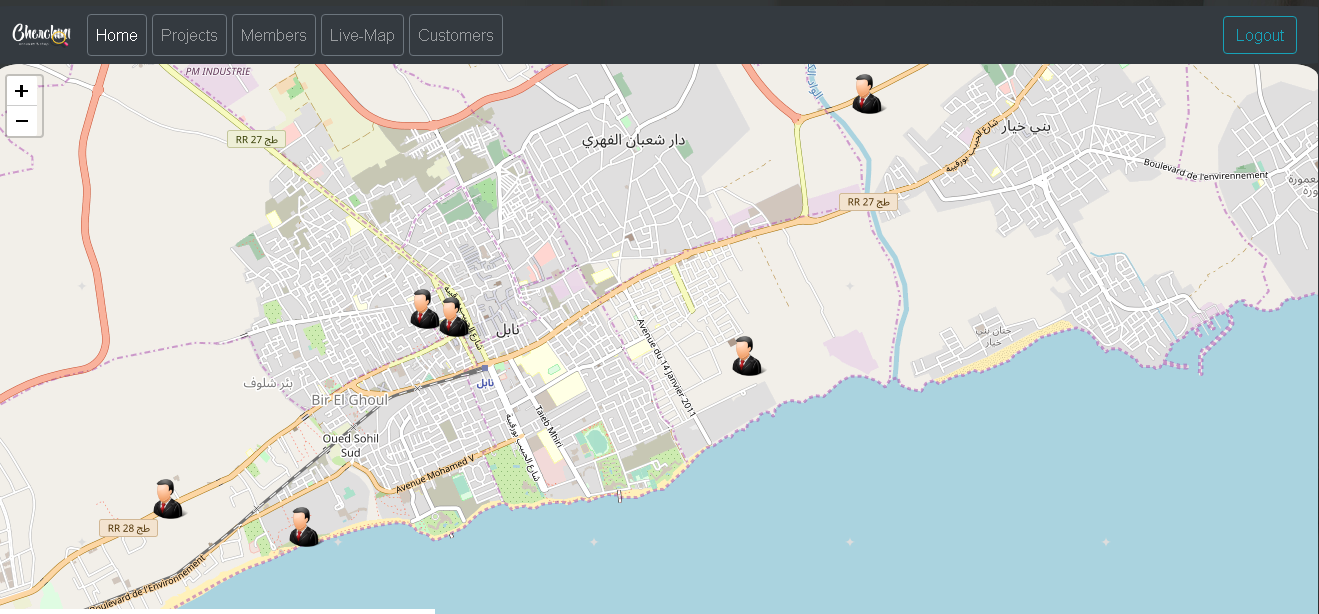
\includegraphics[width=15cm,height=10cm]{./figures/pres/map.png}
\caption{Carte g\'{e}ographique.}
\end{figure}

